\chapter{IMPLEMENTATION}

\section{Working}
\noindent{
    The application is made using \textit{Next JS} which offers both frontend and backend fetaures. The frontend state management is done using \textit{Redux} and \textit{Redux-thunk}. The database we use is \textit{MongoDB} along with \textit{Mongoose} for better schema management.To faclilate login we use \textit{Next Auth} along with  \textit{Bcrypt} for hashing of password while storing in the database. We are using \textit{The Infura API suite} which provides instant access over HTTPS and WebSockets to the Ethereum network. We are also working on \textit{Rinkeby test network} which gives us free ethers to test our application. This applicant is hosted on \textit{Vercel} and can be accessed with the address\\ \url{https://pramanit.vercel.app/}
}
    \subsection{User Module}
    \noindent{The user can register on our platform using email or Gmail sign in available to get \textit{JSON Web Token}. Upon loggin in  the user has option to apply for birth as well as death certificate. \\
    
    For applying the user needs to fill in details and upload attested copies as needed by the Government. These copies are uploaded to \textit{Cloudinary} and urls will be sent to the backend. The form responses are validated by \textit{Formik} using the \textit{Yup schema} and submitted to the  municipality for further processing.\\
    
    Assuming all the documents were correct and the municipality has issued you the certificate, it shall be visible on your dashboard. You can now view the certificate as well as share it with other indivisuals. While generating the pdf of you certficate the ipfs hash id is verified to be present to be on the blockchain. Once confirmed presence the data is accesses from the \textit{Web3Storage} and decrypted. This data using pdf generators is made into pdf as per format approved by the Government\\

    For sharing the certificate the user has 2 options:
        \begin{itemize}
            \item \textbf{Time Based Link}\\
            Select the time duration for which you want to share the certificate. A unique link shall be generated which can be shared across with the desired parties.
            \item \textbf{Direct Third Party}\\
            There is a predefined list of third parties registered on our platform. Select from this list to directly give access to the desired party. This certificate will directly available on their dashboard.\\
        \end{itemize}
        If the application is not approved then the user shall receive a rejection mail stating the reason for rejection. The user can re\-apply for the certicates rectifying the errors. Again the same process of application shall follow.
    }
\subsection{Municipality Module}
\noindent{The municipality recieves applications for both birth and death. The user has an option to accept as well as reject any application.\\

Assuming the case for accepting the application, the user verifies all the uploaded documents and data entered. Now on clicking the issue button the data along the municipality details will be sent to the backend where it will be \textit{encrypted} and added to the \textit{IPFS} using the \textit{Web3Storage}. Once the client recieves the IPFS hash from the backend, the \textit{Metamask wallet} of the municipality will recieve a notification to pay the neceessary gas fees for the transaction to be completed. As the client pays the fees and miners process the data, this data will be added to \textit{Ethereum} to generate the transaction id. The hash id and transaction id are both stored in the \textit{MongoDb database} for further reference.\\

If the municipality wishes to reject an application needs to clearly state the reason for rejection which will trigger a mail to the applicant and reopen the portal for reapplication. \\

The dashboard has record of all the issued, reajected as pending applications. The dashboard also allows the municipality to modify few of its details.
}

\subsection{Time Based Access}
\noindent{Once the third party navigates to the link, using the query parameters the application will get the IPFS hash and verify its presence over the blockchain to present the decrypted certificate in the form of a pdf.}

\subsection{Super Admin Module}
\noindent{The topmost authority which has power to add municipalities to the network. Unless the municipality is added to the network it cannot add new certificates. The super admin is usually the owner of the smart contract and has special access rights in the smart contract. Added to this registering of third party agents which can directly get access to certificate instead of link is also managed by the superadmin.}

\section{Technologies Used}
    \subsection*{Next Js}
    \noindent{The React Framework for Production built together with Google and Facebook.Next.js gives you the best developer experience with all the features you need for production: hybrid static \& server rendering, TypeScript support, smart bundling, route pre-fetching, and more. Next.js powers the biggest websites like Patreon, for use cases in e-commerce, travel, news, and marketing. No config needed. Next.js has all the tools you need to make the Web. Faster.
    }

    \subsection*{Redux}
    \noindent{Redux helps you write applications that behave consistently, run in different environments (client, server, and native), and are easy to test.Redux solves this problem by managing application's state with a single global object called Store. Redux fundamental principles help in maintaining consistency throughout your application, which makes debugging and testing easier.}

    \begin{lstlisting}
        export function addToken(payload) {
            return function (dispatch) {
              dispatch({type: TOKEN_RECIEVED, payload});
            };
          }          
    \end{lstlisting}

    \noindent{Reducers are functions that take the current state and an action as arguments, and return a new state result. In other words, (state, action) =\> newState.
    }

    \begin{lstlisting}
        import {TOKEN_EXPIRED, TOKEN_RECIEVED} from "../types.js";
        const initialState = {token: null};
        export default function reducer(state = initialState, action) {
        switch (action.type) {
            case TOKEN_RECIEVED:
            return {token: action.payload};
            default:
            return state;
        }
    }
    \end{lstlisting}
      
\noindent{The Redux store brings together the state, actions, and reducers that make up your app. The store has several responsibilities:

\begin{itemize}
    \item Holds the current application state inside
    \item Allows access to the current state via store.getState();
    \item Allows state to be updated via store.dispatch(action);
    \item Registers listener callbacks via store.subscribe(listener);
    \item Handles unregistering of listeners via the unsubscribe function returned by store.subscribe(listener).
\end{itemize}}

\begin{lstlisting}
        import {createStore, applyMiddleware} from "redux";
        import {composeWithDevTools} from "redux-devtools-extension";
        import thunk from "redux-thunk";
        import rootReducer from "./reducers";

        export default function initializeStore(initialState = {}) {
        return createStore(
            rootReducer,
            initialState,
            composeWithDevTools(applyMiddleware(thunk))
        );
        }
\end{lstlisting}

\subsection*{Cloudinary}
\noindent{Cloudinary is an end-to-end image- and video-management solution for websites and mobile apps, covering everything from image and video uploads, storage, manipulations, optimizations to delivery.With Cloudinary, you can easily upload images and videos to the cloud and automate smart manipulations of those media without installing any other software. Cloudinary then seamlessly delivers your media through a fast content delivery network (CDN), optimized with the industry’s best practices.Additionally, Cloudinary offers comprehensive APIs and administration capabilities, which you can easily integrate with your web and mobile apps.
}

\begin{lstlisting}
        cloudinary.v2.uploader.upload(
            result.files.file.filepath,
            {pages: true},
            (err, result) => {
            console.log(result, err);
            if (result != undefined) {
                res.status(200).send(result);
            } else {
                res.status(400).send("Upload Failed", err);
            }
            }
        ); 
\end{lstlisting}

\subsection*{JSON Web Token}
\noindent{JSON Web Token (JWT) is a proposed Internet standard for creating data with optional signature and/or optional encryption whose payload holds JSON that asserts some number of claims. The tokens are signed either using a private secret or a public/private key.
Secret Or PrivateKey is a string, buffer, or object containing either the secret for HMAC algorithms or the PEM encoded private key for RSA and ECDSA. In case of a private key with passphrase an object { key, passphrase } can be used (based on crypto documentation), in this case be sure you pass the algorithm option.
}

\begin{lstlisting}
        const token = jwt.sign({_id: user._id}, "mysecret", {
                    expiresIn: "7d",
                    });
\end{lstlisting}

\subsection*{Bcrypt library}
\noindent{The bcrypt npm package is one of the most used packages to work with passwords in JavaScript. Storing plain text passwords is one of the worst habits of our time. Don't store plain text passwords, instead use passwords hashing.
}
\begin{lstlisting}
        bcrypt.hash(newUser.password, saltRound, (err, hash) => {//store the hash to the db})
        bcrypt.compare(req.body.password, user.password).then((isMatch) => {
                    if (isMatch) {
                        //login
                        }
                    })
\end{lstlisting}

\subsection*{Mongoose}
\noindent{Mongoose is an Object Data Modeling (ODM) library for MongoDB and Node.js. It manages relationships between data, provides schema validation, and is used to translate between objects in code and the representation of those objects in MongoDB.
}
\begin{lstlisting}
        await mongoose.connect(
        process.env.MONGO_URI,
        {
        useUnifiedTopology: true,
        useNewUrlParser: true,
        });
\end{lstlisting}

\subsection*{Formik}
\noindent{Formik is a small group of React components and hooks for building forms in React and React Native. It helps with the three most annoying parts:}
\begin{itemize}
    \item Getting values in and out of form state
    \item Validation and error messages
    \item Handling form submission
\end{itemize}
\noindent{By co-locating all of the above in one place, Formik keeps things organized--making testing, refactoring, and reasoning about your forms a breeze.
}
\begin{lstlisting}
        import {Formik, Form} from "formik";
        <Formik
            initialValues={{...INITIAL_FORM_STATE}}
            validationSchema={FORM_VALIDATION}
            onSubmit={onSubmit}
            >
            <Form>
                <InputField title="Email" name="email" />
                    <Button>Login</Button>
            </Form>
        </Formik>    
\end{lstlisting}

\subsection*{Yup}
\noindent{Yup is a JavaScript schema builder for value parsing and validation. Define a schema, transform a value to match, validate the shape of an existing value, or both. Yup schemas are extremely expressive and allow modeling complex, interdependent validations, or value transformations.
Yup's API is  leaner and built with client-side validation as its primary use-case. Yup separates the parsing and validating functions into separate steps. cast() transforms data while validate checks that the input is the correct shape. Each can be performed together (such as HTML form validation) or separately (such as deserializing trusted data from APIs).
}
\begin{lstlisting}
        const FORM_VALIDATION = Yup.object().shape({
            username: Yup.string().required("Username is Required."),
            email: Yup.string().email("Invalid email.").required("Email is Required."),
        });      
\end{lstlisting}

\subsection*{Axios}
\noindent{Axios is a promise based HTTP client for the browser and Node.js. Axios makes it easy to send asynchronous HTTP requests to REST endpoints and perform CRUD operations. It can be used in plain JavaScript or with a library such as Vue or React.\\
These are basic methods for generating requests in axios.
}
\begin{lstlisting}
        axios.request(config)
        axios.get(url[, config])
        axios.post(url[, data[, config]])
        axios.put(url[, data[, config]])      
\end{lstlisting}

\subsection*{Vercel}
\noindent{Vercel (formerly known as ZEIT) is a cloud platform that enables developers to host websites and web services that deploy instantly, scale automatically, and require no supervision.Vercel is also a parent company of the Next.js framework. Vercel is the best place to deploy any frontend app. Start by deploying with zero configuration to our global edge network. Scale dynamically to millions of pages without breaking a sweat.The Vercel platform makes it a collaborative experience with deploy previews for every code change, by seamlessly integrating with GitHub, GitLab, and Bitbucket. It also handles SSL certification.
}

\begin{itemize}
    \item Fast Refresh
    \item Flexible Data Fetching
\end{itemize}

\url{https://pramanit.vercel.app/}

\subsection*{Solidity}
\noindent{Solidity is a brand-new programming language created by Ethereum which is the second-largest market of cryptocurrency by capitalization, released in the year 2015 led by Christian Reitwiessner. Some key features of solidity are listed below: }

\begin{itemize}
    \item Solidity is a high-level programming language designed for implementing smart contracts.
    \item It is a statically-typed object-oriented(contract-oriented) language.
    Solidity is highly influenced by Python, c++, and JavaScript which runs on the Ethereum Virtual Machine(EVM).
    \item Solidity supports complex user-defined programming, libraries and inheritance.
    \item Solidity is the primary language for blockchains running platforms.
    \item Solidity can be used to create contracts like voting, blind auctions, crowdfunding, multi-signature wallets, etc.
\end{itemize}

\subsection*{Ethereum}
\noindent{Ethereum is a decentralized open-source platform based on the blockchain domain, used to run smart contracts i.e. applications that execute the program exactly as it was programmed without the possibility of any fraud, interference from a third party, censorship, or downtime. It serves a platform for nearly 2,60,000 different cryptocurrencies. Ether is a cryptocurrency generated by ethereum miners, used to reward for the computations performed to secure the blockchain. }

\subsection*{Smart Contract}
\noindent{Smart contracts are high-level program codes that are compiled to EVM bytecode and deployed to the ethereum blockchain for further execution. It allows us to perform credible transactions without any interference of the third party, these transactions are trackable and irreversible. Languages used to write smart contracts are Solidity (a language library with similarities to C and JavaScript), Serpent (similar to Python, but deprecated), LLL (a low-level Lisp-like language), and Mutan (Go-based, but deprecated).}

\begin{lstlisting}
        contract Muncipality{
        address public owner;
        UserData[] public allUser;

        struct UserData{
            uint uid;
            string BirthHash;
            string DeathHash;
            uint length;
        }

        mapping (uint=>bool) public isPresent;
        uint public UserLength=0;
        constructor() public{
            onwer=msg.sender;
        }
        modifier onlyOwner{
            require(msg.sender==onwer);
        }
        function CheckPresence(uint uid) public returns(bool){
            if(isPresent[uid]==true) return true;
            return false;
        }
        
            function AddUserBirthHash(uint munId,uint uid,string memory _BirthHash) public returns(bool){
                if(CheckPresence(munId)){
                UserDara memory newUser=UserData({
                    uid:uid,
                    BirthHash:_BirthHash,
                    DeathHash:' ',
                    length:UserLength
                });
                allUser.push(newUser);
                return true;
            }
                else{return false }
            } 
        }

\end{lstlisting}

\subsection*{Truffle}
\noindent{A world class development environment, testing framework and asset pipeline for blockchains using the Ethereum Virtual Machine (EVM), aiming to make life as a developer easier. Truffle is clearly a smart contract development environment. This environment has several wonderful features that benefit dApp developers a lot. Truffle is the ecosystem's development, asset pipeline, and testing framework. Truffle is a popular Ethereum dApp development framework with a significant community. Also, Truffle uses the EVM as a foundation and aims to make smart contract creation easier and more accessible.\\
Truffle has various advantages:
}
\begin{itemize}
    \item Truffle helps manage the artifacts of any smart contracts used in your dApps. 
    \item Automated Contract Testing
    \item Scriptable Migration and Deployment
    \item Truffle manages your artifacts, allowing you to focus on other things.
    \item Truffle has an interactive console where you can access all your Truffle commands and contracts.
\end{itemize}

\subsection*{Ganache}
\noindent{A personal blockchain for Ethereum development you can use to deploy contracts, develop your applications, and run tests. It is available as both a desktop application as well as a command-line tool (formerly known as the TestRPC). Ganache is available for Windows, Mac, and Linux. Ganache is a tool for creating a local Ethereum blockchain. The blockchain may be used in all stages of development, making it very beneficial. As we set up our local blockchain, Ganache helps us to safely install, create, and test our dApps. We should use a local blockchain while designing applications for two reasons. First, we can save money, and second, we can save time.Uploading contracts to an authoritative chain like Ethereum mainnet costs gas. This can be problematic because of the high and unpredictable fees. As a result, uploading contracts that are still not operating might be quite costly.}

\subsection*{Infura}
\noindent{Infura is a blockchain development suite that provides application programming interfaces (APIs) and developer tools. Moreover, Infura provides fast and reliable access to the Ethereum network to enable developers to build sophisticated next-generation software and Web3 applications that scale to meet user demand.
Infura offers enterprise-ready infrastructure using a distributed cloud-hosted network of nodes. This removes much of the friction associated with the development and ownership of proprietary computing and storage facilities.}

\subsection*{Etherscan}
\noindent{Etherscan is a blockchain explorer platform for the Ethereum blockchain. You can use this free tool to view any past transaction, wallet, smart contract, NFT, and anything else you may want to view in the history of Ethereum. There are similar products for other blockchains as well.\\

You can view new transactions and blocks on the Etherscan homepage.That means you can find your wallet and historical transactions, but you would have to go to your cryptocurrency exchange or wallet provider to use Ether or enter a transaction.
}

\subsection*{Metamask}
\noindent{MetaMask is a browser plugin that serves as an Ethereum wallet, and is installed like any other browser plugin. Once it's installed, it allows users to store Ether and other ERC-20 tokens, enabling them to transact with any Ethereum address.The ERC-20 token standard allows developers to create their own tokens on the Ethereum network. It has provided an easier route for companies to develop blockchain products instead of building their own cryptocurrency.
By connecting MetaMask to Ethereum-based dapps, users can spend their coins in games, stake tokens in gambling applications, and trade them on decentralized exchanges (DEXs).}

\subsection*{Web3.Storage}
\noindent{Web3.Storage, a simple interface for developers to store and retrieve data from Filecoin’s decentralized storage network! Web3.Storage: which will remain free indefinitely gives developers an easy avenue to build applications with redundant, decentralized storage and secure, content addressed data.
Web3.Storage contains two main components:
\begin{itemize}
    \item A service that stores data redundantly across multiple Filecoin miners and the public IPFS network, provides information about where the data is stored, and retrieves data by CID.
    \item An HTTP endpoint, JavaScript client library, and web UI for interacting with the service.
\end{itemize}
How Does It Work?\\
Behind the scenes, content that is sent to Web3.Storage is persistently stored across a network of storage providers on Filecoin and pinned redundantly on IPFS. Together, Filecoin and IPFS endow content, data, and applications with content addressability and persistence. Content addressability enables immutable links that are based on the content itself (CIDs), rendering information impossible to change, edit, or compromise without leaving a traceable record of tampering. Persistence ensures the data stored via this service will remain intact and available backed by the robust economic model of Filecoin and verifiable proofs regarding the stored data’s integrity.}

\subsection*{Redux-thunk}
\noindent{Redux Thunk is middleware that allows you to return functions, rather than just actions, within Redux. This allows for delayed actions, including working with promises.
One of the main use cases for this middleware is for handling actions that might not be synchronous, for example, using axios to send a GET request. Redux Thunk allows us to dispatch those actions asynchronously and resolve each promise that gets returned.}

\subsection*{Ncrypt-js}
\noindent{Ncrypt.Js is a lightweight javascript data encryption and decryption library. This library implements the nodejs default crypto functionality as a mid-channel cipher in addition to a simple and elegant custom data encoding and encryption algorithm.
Encryption and decryption of JavaScript object literal has never been simpler than this.
To encrypt and decrypt JavaScript object literal, simply use encrypt() and decrypt() function from an instance. This will use the AES-CBC encryption algorithm.
}

\subsection*{NextAuth}
\noindent{NextAuth.js is a complete open source authentication solution for Next.js applications.It is designed from the ground up to support Next.js and Serverless.}
\begin{itemize}
    \item Easy
    \item Flexible
    \item Secure
\end{itemize}

\subsection*{Rinkeby network}
\noindent{Rinkeby is an Ethereum testnet (or test network). Testnets are typically used by developers to run "tests" for their application or software. Currency on testnet is valueless. Rinkeby testnet, unlike Ethereum mainnet, is a proof-of-authority network, as opposed to a proof-of-work network like Ethereum mainnet.}

\subsection*{Rinkeby Faucet}
\noindent{An Ethereum faucet is a developer tool to get testnet Ether (ETH) in order to test and troubleshoot your decentralized application or protocol before going live on Ethereum mainnet, where one must use real Ether. Most faucets require social authentication (e.g. Twitter post or login confirming you are a real human) or place you in a queue to wait for a testnet token through the faucet. The Alchemy Rinkeby faucet is free, fast, and does not require authentication, though you can optionally login to Alchemy to get an increased drip.}

\subsection*{Test Net Token}
\noindent{Testnet tokens are a test currency that allows you to test your Ethereum application before going live on mainnet. Testnet tokens can be used in place of mainnet Ether tokens on testnets like Rinkeby.}

\section{Website Design}
    \begin{figure}[H]
        \centering
        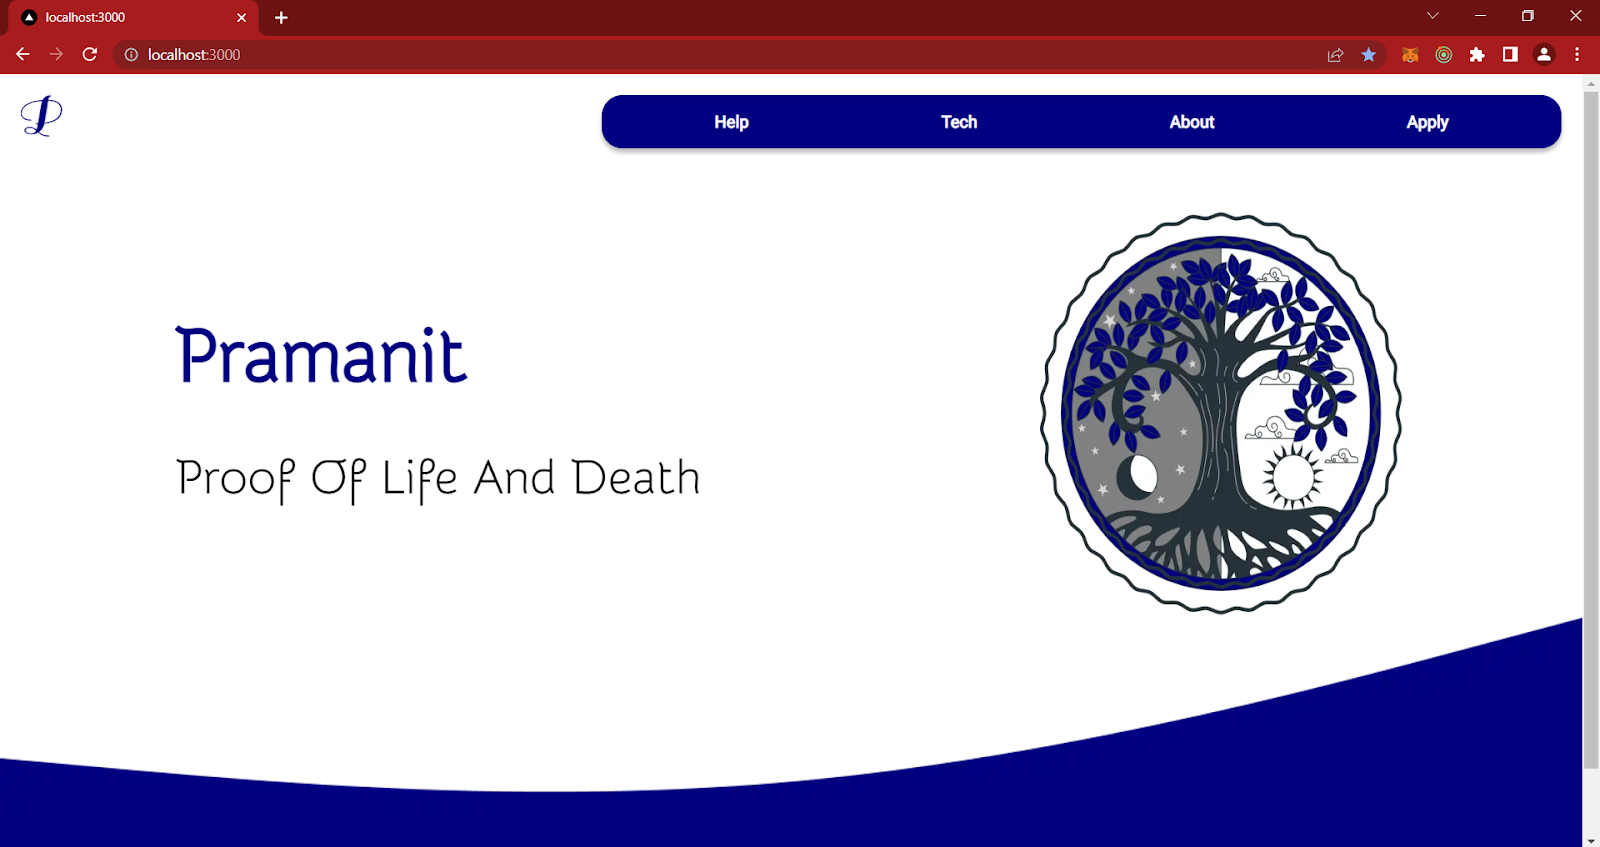
\includegraphics[width=\textwidth]{imgs/landingpage.png}
        \caption{Landing page of the project website}
        \label{fig:Landing page of the project website}
        \end{figure}

    \begin{figure}[H]
        \centering
        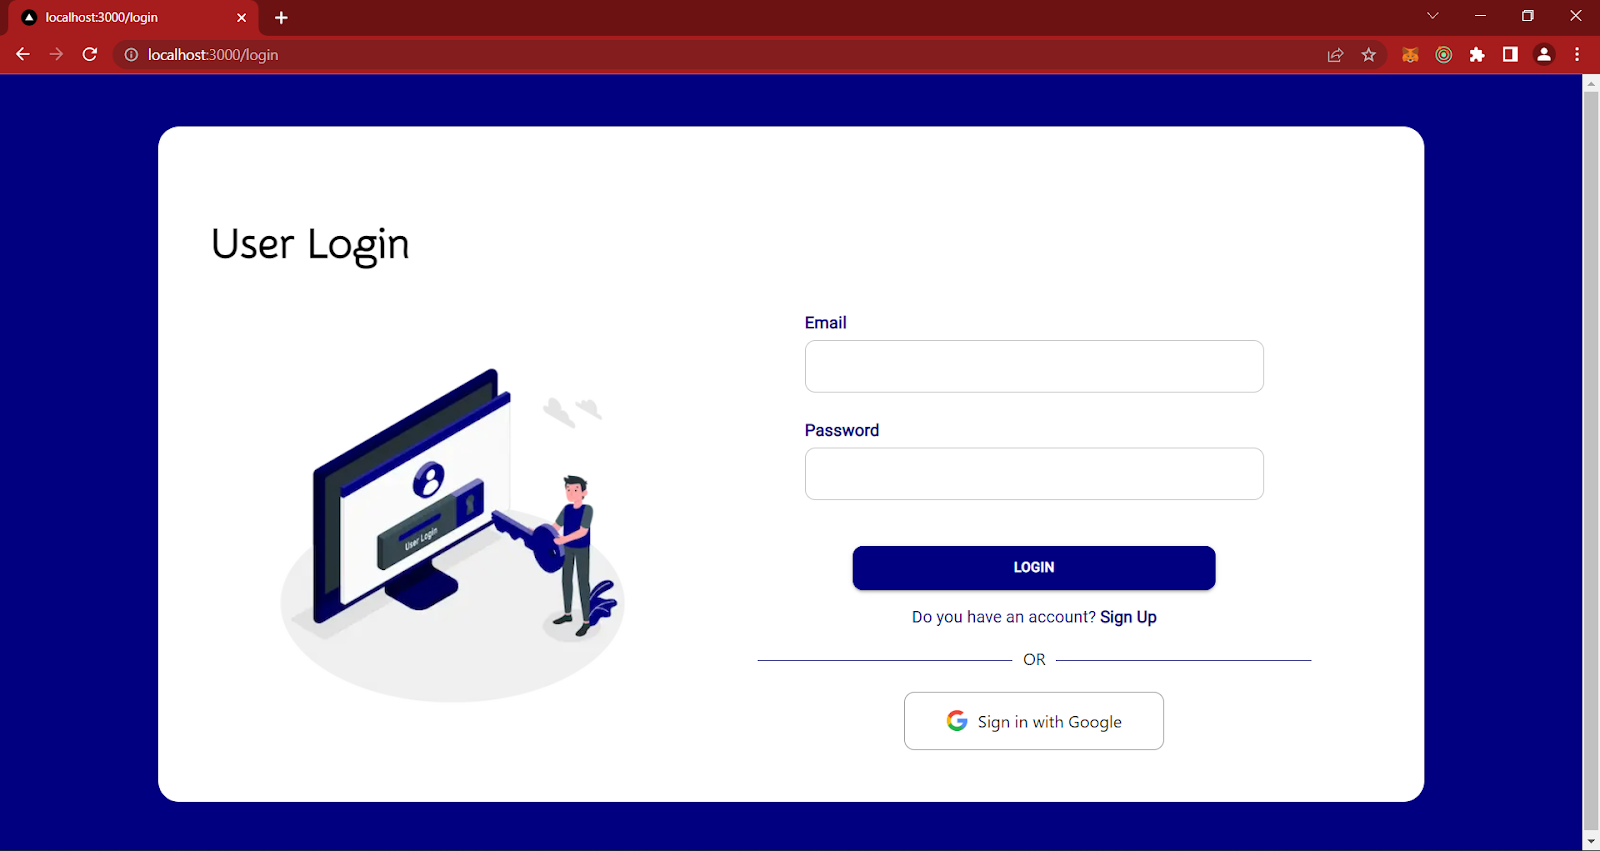
\includegraphics[width=\textwidth]{imgs/loginpage.png}
        \caption{Login page of the project}
        \label{fig:Login page of the project}
        \end{figure}

    \begin{figure}[H]
        \centering
        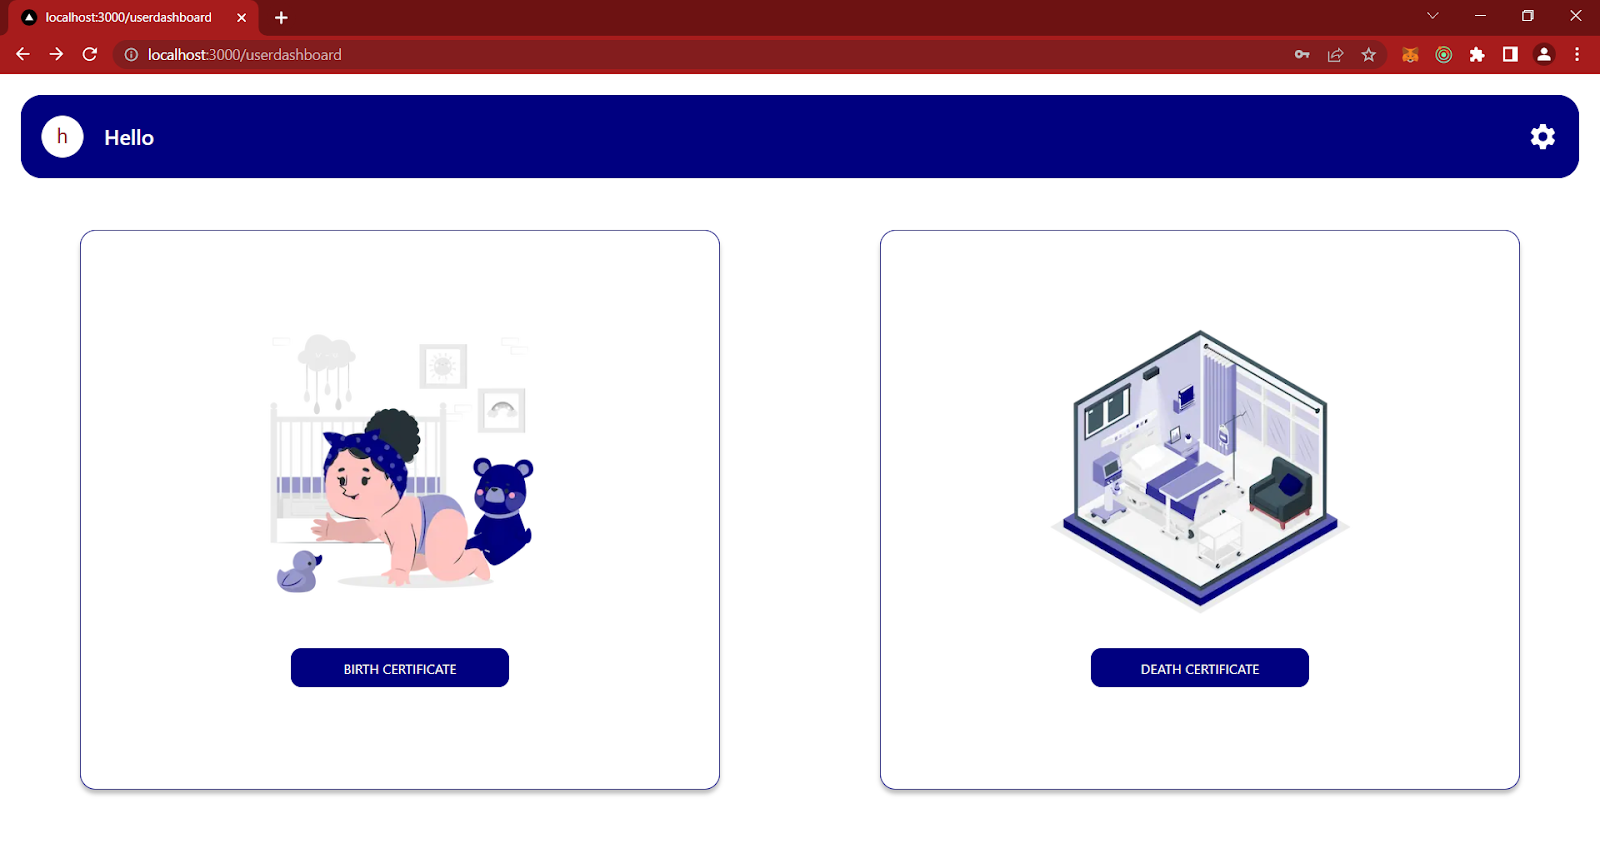
\includegraphics[width=\textwidth]{imgs/userdashboardpage.png}
        \caption{Userdashboard page of the project}
        \label{fig:Userdashboard page of the project}
        \end{figure}

    \begin{figure}[H]
        \centering
        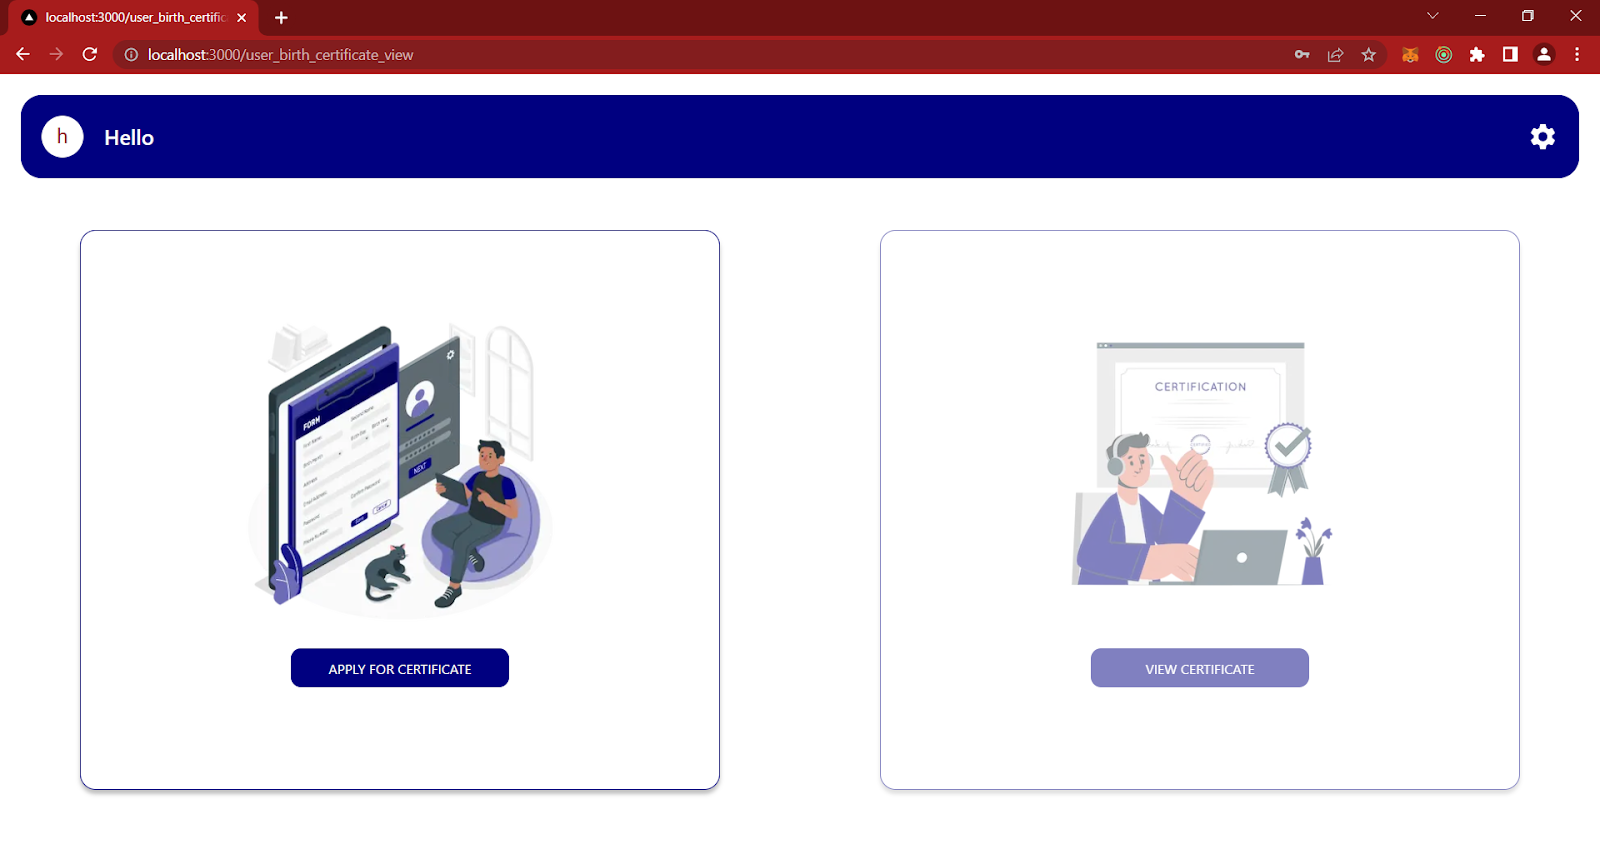
\includegraphics[width=\textwidth]{imgs/birthdashboardpage.png}
        \caption{Birth certificate section page of the project}
        \label{fig:Birth certificate section page of the project}
        \end{figure}

    \begin{figure}[H]
        \centering
        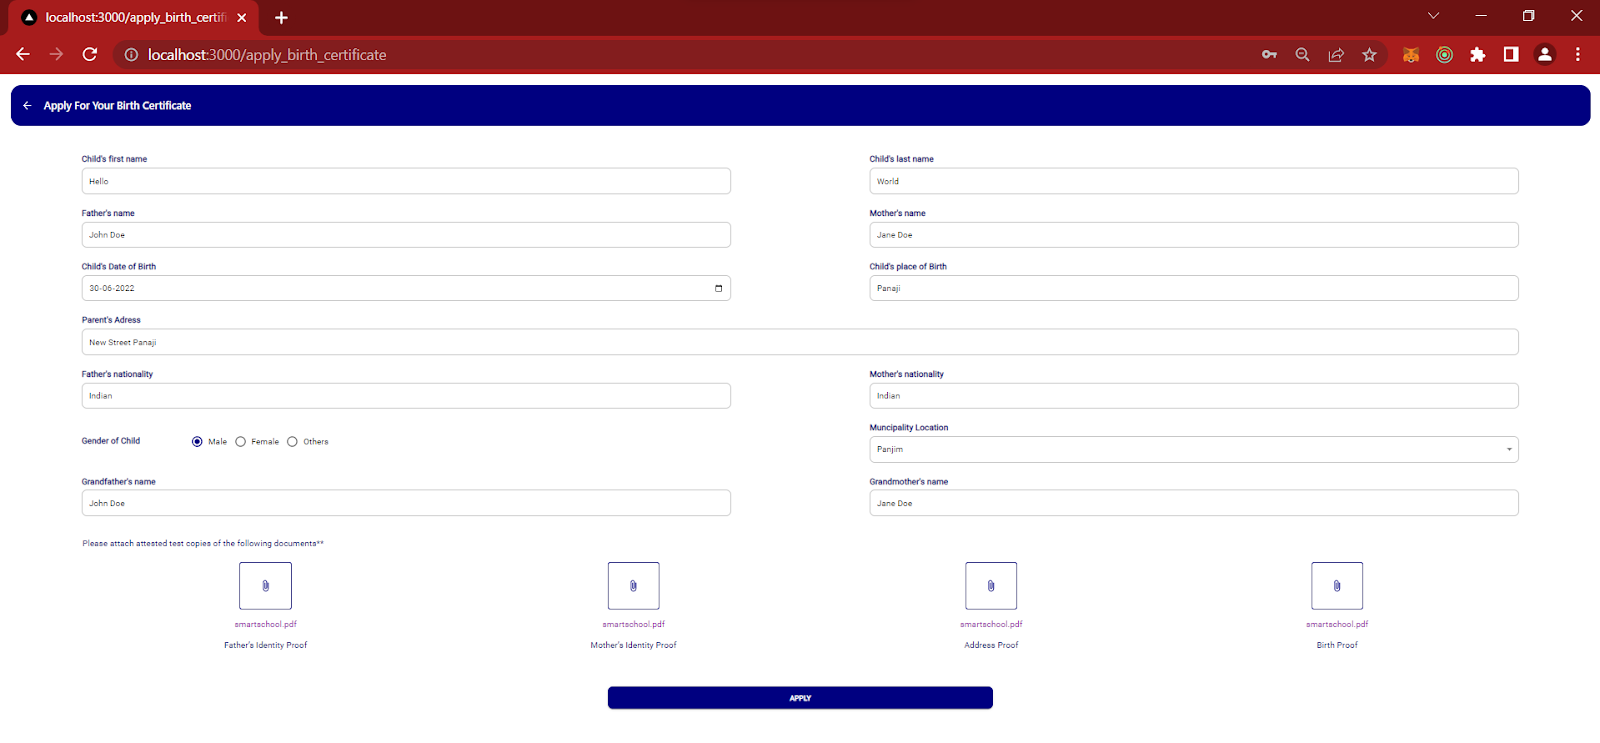
\includegraphics[width=\textwidth]{imgs/applycertificatepage.png}
        \caption{Apply certificate page of the project}
        \label{fig:Apply certificate page of the project}
        \end{figure}

    \begin{figure}[H]
        \centering
        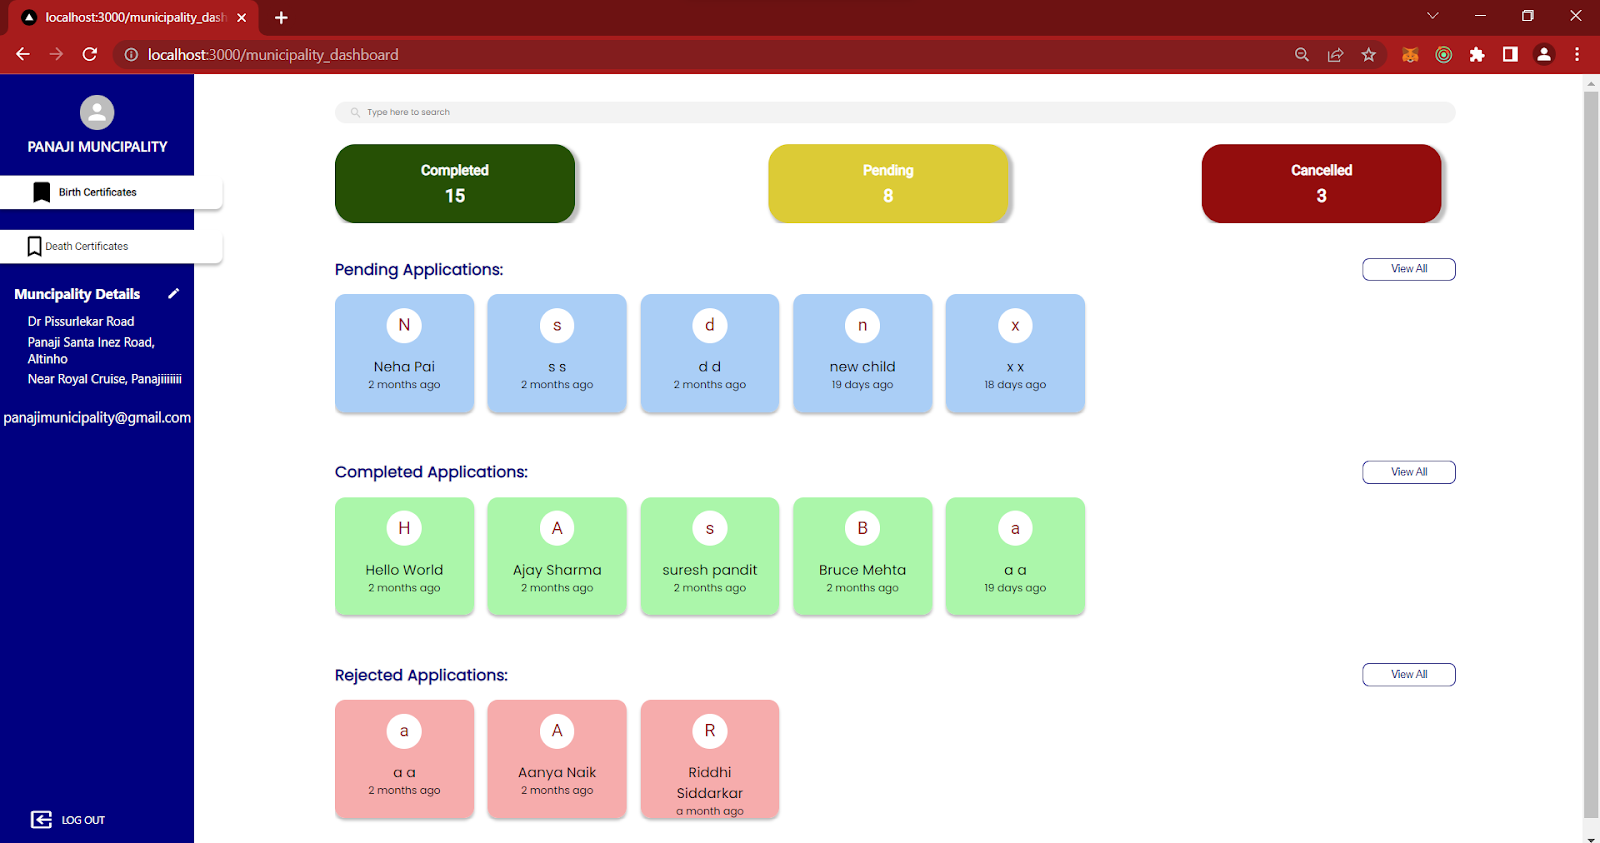
\includegraphics[width=\textwidth]{imgs/municipalitypage.png}
        \caption{Municipality dashboard page of the project}
        \label{fig:Municipality dashboard page of the project}
        \end{figure}

    \begin{figure}[H]
        \centering
        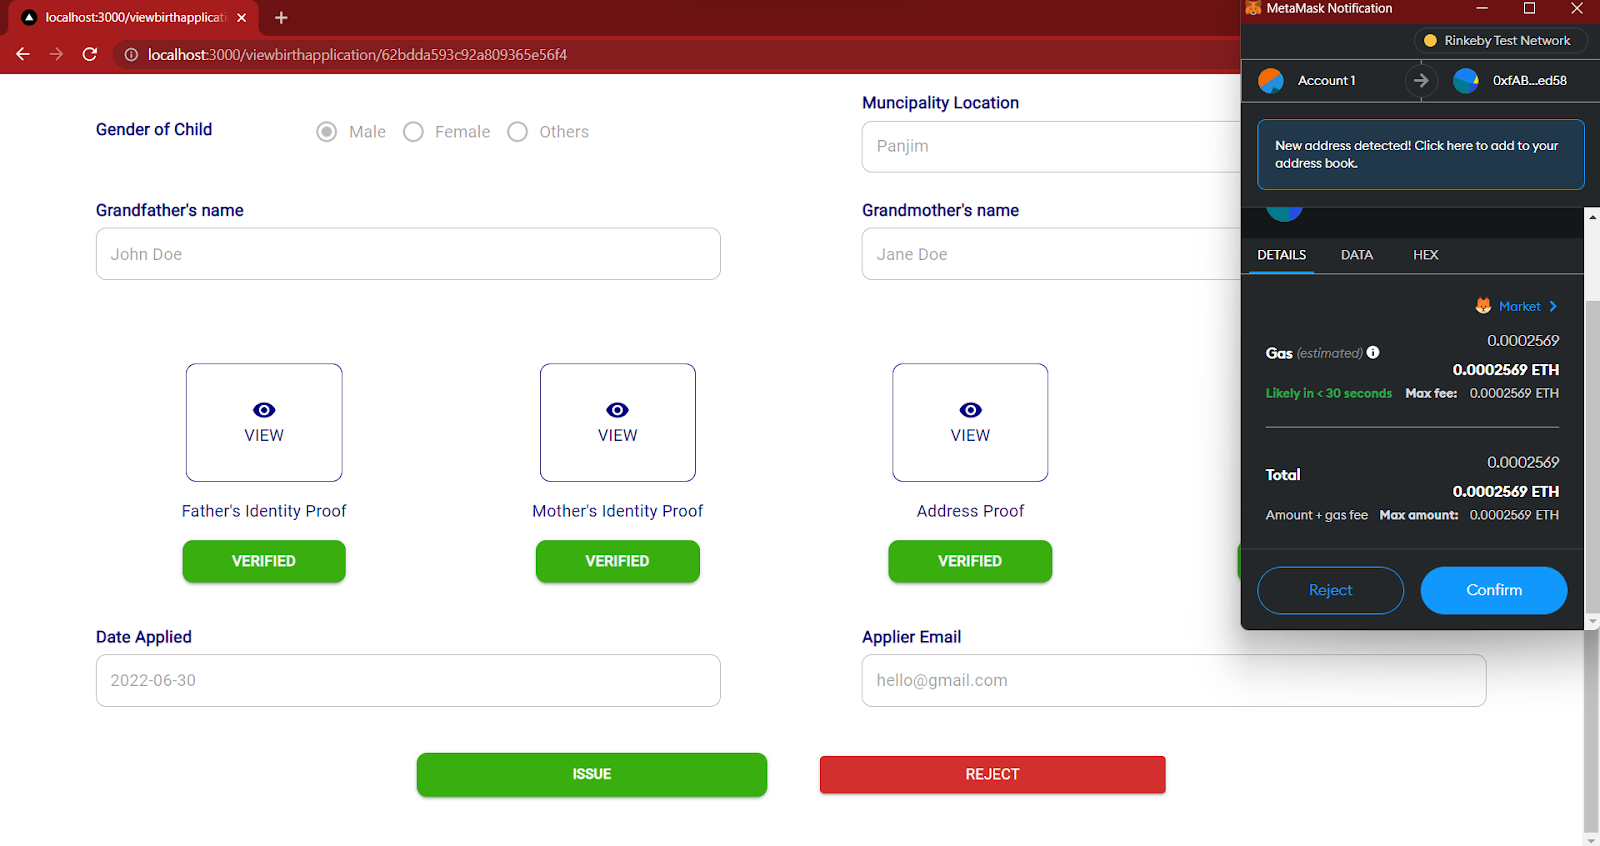
\includegraphics[width=\textwidth]{imgs/grantingcertificate.png}
        \caption{Payment of gas fees while issuing a certificate by municipality}
        \label{fig:Payment of gas fees while issuing a certificate by municipality}
        \end{figure}

    \begin{figure}[H]
        \centering
        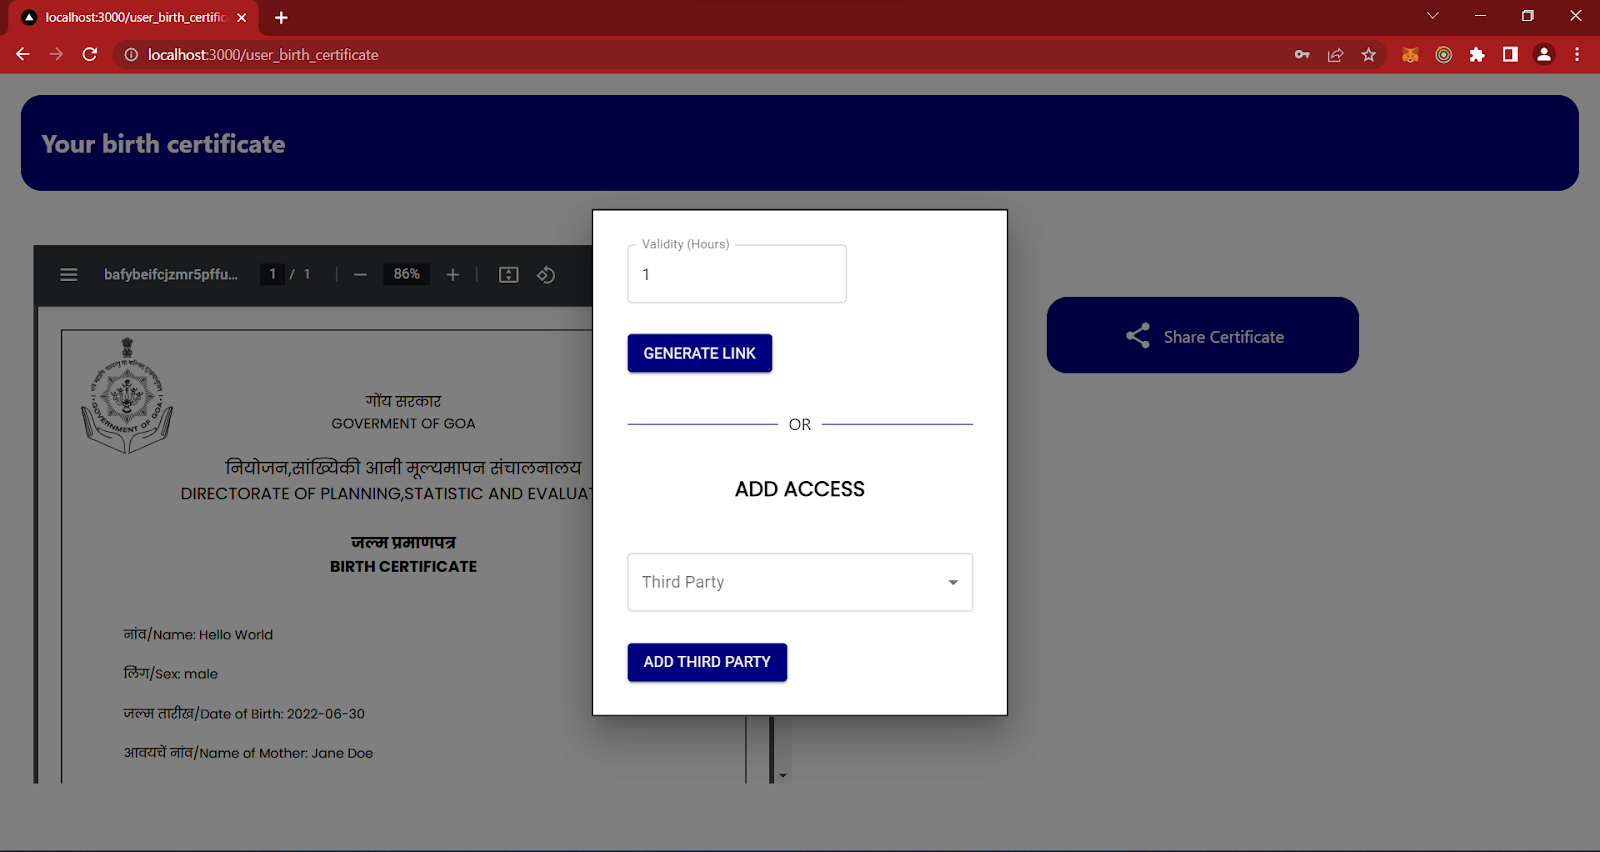
\includegraphics[width=\textwidth]{imgs/adding3rdpartyacess.png}
        \caption{Adding third party access to the certificate}
        \label{fig:Adding third party access to the certificate}
        \end{figure}

\section{Database Details}
    \subsection{Municipality Schema}
    \begin{lstlisting}
        new mongoose.Schema({
            name: {
                type: String,
            },
            email: {
                type: String,
            },
            password: {
                type: String,
            },
            addressLine1: {
                type: String,
            },
            addressLine2: {
                type: String,
            },
            addressLine3: {
                type: String,
            },
            code: {
                type: String,
            },
            pincode: {
                type: String,
            },
            accessToken: {type: String},
            resetToken: {type: String},
            metamaskAddress:{type:String},
            issuingauthoritysign: {
                type: String,
            },
            issuingauthorityname: {
                type: String,
            },
            municipalityseal: {
                type: String,
            },
            cheifregistrarsign: {
                type: String,
            },
        })
    \end{lstlisting}

    \subsection{User Schema}
    \begin{lstlisting}
        new mongoose.Schema({
            username: {
                type: String,
            },
            email: {
                type: String,
            },
            password: {
                type: String,
            },
            birthIpfsHash: {
                type: String,
                default: "",
            },
            birthTransactionId: {
                type: String,
                default: "",
            },
            deathIpfsHash: {
                type: String,
                default: "",
            },
            deathTransactionId: {
                type: String,
                default: "",
            },
            accessToken: {type: String},
            resetToken: {type: String},
            birthCertificateStatus: {
                type: Number,
                default: 0,
            },
            deathCertificateStatus: {
                type: Number,
                default: 0,
            },
        })
    \end{lstlisting}

    \subsection{Birth Application Schema}
    \begin{lstlisting}
        new mongoose.Schema({
            childFirstName: {
                type: String,
            },
            childLastName: {
                type: String,
            },
            fatherName: {
                type: String,
            },
            motherName: {
                type: String,
            },
            dateOfBirth: {
                type: Date,
            },
            placeOfBirth: {
                type: String,
            },
            address: {
                type: String,
            },
            fatherNationality: {
                type: String,
            },
            motherNationality: {
                type: String,
            },
            gender: {
                type: String,
            },
            grandFatherName: {
                type: String,
            },
            grandMotherName: {
                type: String,
            },
            muncipalityLocation: {
                type: String,
            },
            fatherIdentityProof: {
                type: String,
            },
            motherIdentityProof: {
                type: String,
            },
            addressProof: {
                type: String,
            },
            birthProof: {
                type: String,
            },
            createdAt: {
                type: Date,
                default: new Date(),
            },
            issued: {
                type: Number,
                default: 0,
            },
            applicant_id: {
                type: String,
            },
        });
    \end{lstlisting}

    \subsection{Super Admin schema}
    \begin{lstlisting}
        new mongoose.Schema({
            username: {
                type: String,
            },
            email: {
                type: String,
            },
            password: {
                type: String,
            },
        })
    \end{lstlisting}

    \subsection{Time based certificate schema}
    \begin{lstlisting}
        new mongoose.Schema({
            userid: {
                type: String,
            },
            validTill: {
                type: Date,
            },
            type: {
                type: String,
            },
        })
    \end{lstlisting}

    \subsection{Third Party Schema}
    \begin{lstlisting}
        new mongoose.Schema({
            name: {
                type: String,
            },
            email: {
                type: String,
            },
            password: {
                type: String,
            },
            birthcertificates: {
                type: Array,
                default: [],
            },
            deathcertificates: {
                type: Array,
                default: [],
            },
        })
    \end{lstlisting}    

\section{Cost for certificates}

\textit{Cost of Ethereuem is Rs. 1,66,500 as of 15th August 2022}

\begin{table}[H]
    \normalsize
    \begin{center}
    \begin{tabular}{|m{3.5cm}| m{3.5cm}|m{3.5cm}|m{3.5cm}|}
        \hline
        \textbf{Event} & \textbf{Cost In Ethers} & \textbf{Cost in Rupees}& \textbf{Comments}\\
        \hline
        Contract deploy	& 0.001329 &221.351 &One time transaction\\
        \hline
        Adding Municipality &	0.000207 &	34.464&	Once to add municipality\\
        \hline
        Adding Certificate&0.000343	& 57.031 &Twice per user (Birthcertificate \+ Death Certificate)\\
        \hline
    \end{tabular}  
    \caption{Cost of each transaction on ethereum platform}
    \label{table-example}
    \end{center}
    \end{table}